\newgeometry{total={8in,10.5in},hoffset=0.2in,voffset=0.3in}
%nb: I just messed with the numbers above until it looked okay.  I really don't know what I'm doing. --MT, 4/23/2016
\thispagestyle{empty}
\definecolor{darkblue}{RGB}{0,0,160}
\newpagecolor{darkblue}

\begin{center}
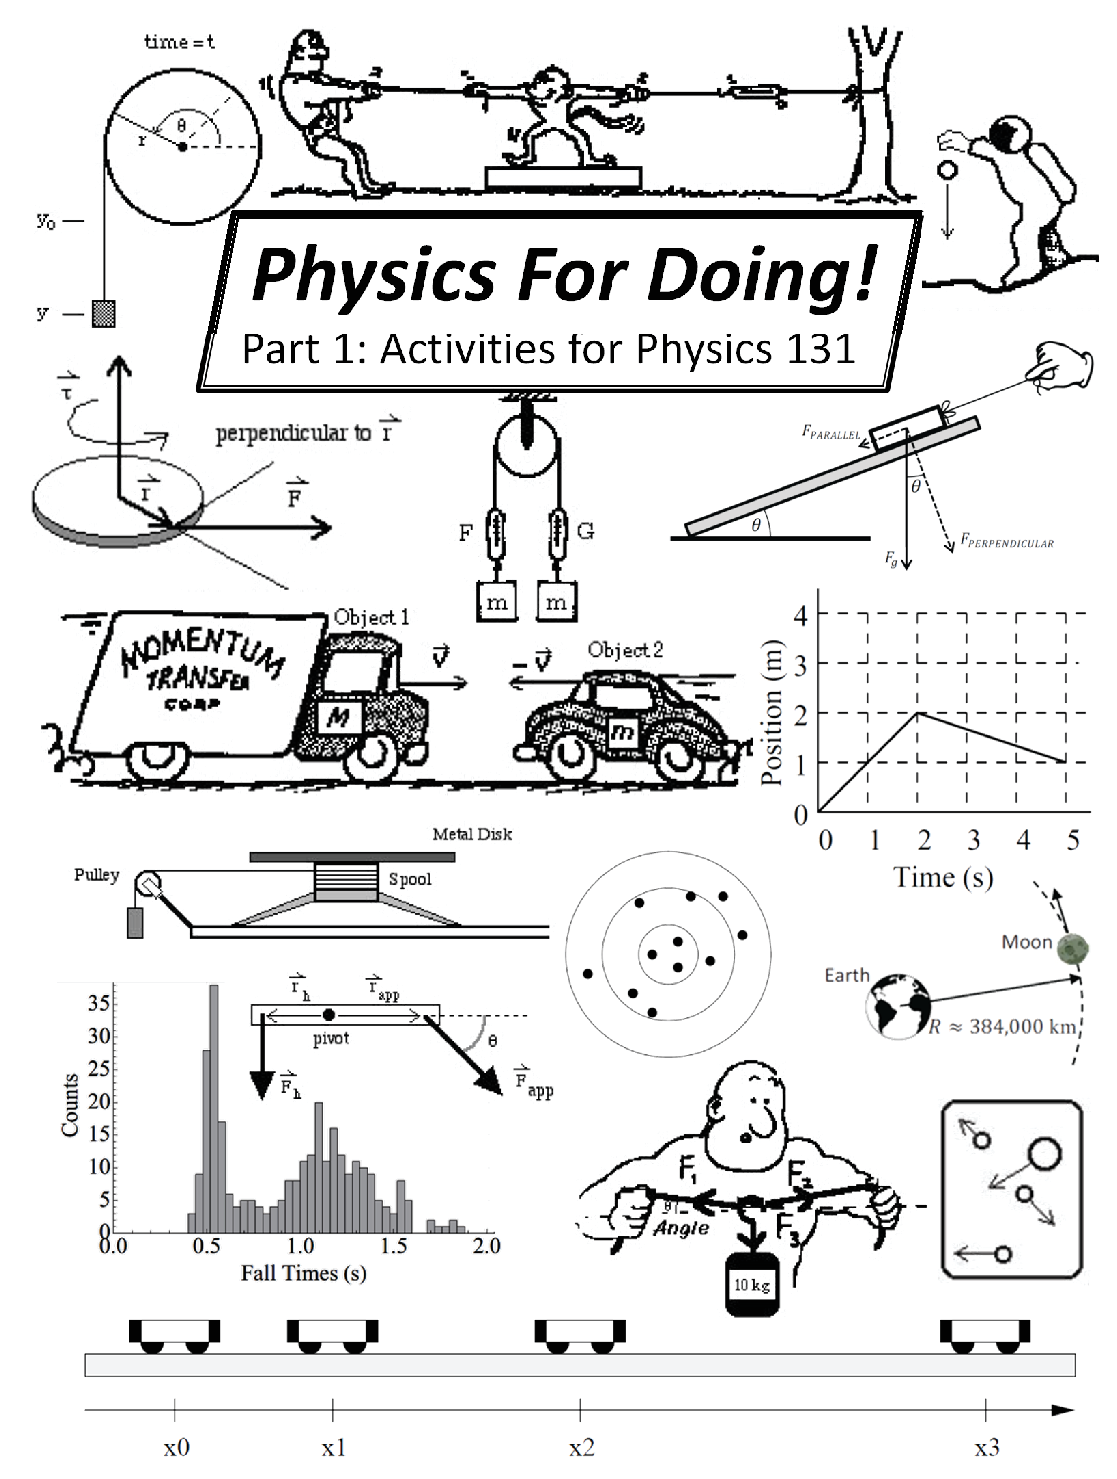
\includegraphics[width=7.3in,trim={0 0 .1cm 0},clip]{131_front_pages/131_front_cover.eps}
\index{color page}
\end{center}
\newpage

\restoregeometry
\restorepagecolor
\thispagestyle{empty}

\
\vfill
\textit{Cover art: Various graphics and diagrams from the activities in this manual.  You'll be doing lots of stuff.}
\pagebreak



\title{Physics For Doing!\\
Part 1: Activities for Physics 131}

\author{Emory F. Bunn, 
Mirela Fetea\footnote{Current address: Germanna Community College, Fredericksburg, VA}, 
Gerard P. Gilfoyle, Henry Nebel, \\
Philip D. Rubin\footnote{Current address: Department of Physics, George Mason University, Fairfax, VA}, 
Jack Singal, Matthew L. Trawick, 
and Michael F. Vineyard\footnote{Current address: Department of Physics, Union College, Schenectady, NY}\\[4pt]
Department of Physics, University of Richmond, VA \\[4pt]
%$^2$Department of Physics, George Mason University, Fairfax, VA \\[4pt]
%$^3$Department of Physics, Union College, Schenectady, NY \\[4pt]
%$^4$Germanna Community College, Fredericksburg, VA 22408
}

\maketitle

\vspace{0.8 in}

%\begin{abstract}

\begin{center}
\large{\textbf{Welcome to Physics 131!}}
\end{center}

The exercises in this manual have been developed to support an investigative
physics course that emphasizes active learning. 
%The units are made up of activities designed to guide your investigations in the laboratory. 
Your written work will consist primarily of documenting
your class activities by filling in the entries in the spaces provided
in the units. The entries consist of observations, derivations, calculations,
and answers to questions. Although you may use the same data and graphs
as your partner(s) and discuss concepts with your classmates, all
entries should reflect your own understanding of the concepts and
the meaning of the data and graphs you are presenting. Thus, each
entry should be written in your own words. It is very important
to your success in this course that your entries reflect a sound understanding
of the phenomena you are observing and analyzing. 

Some of these units
have been taken from the Workshop Physics project at Dickinson College
and the Tools for Scientific Thinking project at Tufts University
and modified for use at the University of Richmond. Others have been
developed locally. 
We wish to acknowledge the support we have received for this project
from the University of Richmond and the Instrumentation and Laboratory
Improvement program of the National Science Foundation. Also, we would
like to thank our laboratory directors for their invaluable technical
assistance.
%\end{abstract}


\newpage
\
\thispagestyle{plain}

\newpage
\
%\setcounter{page}{2} %changed from 1 to 2 on 6/9/15 by MT.  The reason is that in the circuit labs, the odd pages need to be on the right (the fronts of each sheet of paper) and the even pages need to be on the left.  This is critical, because these labs have some pages that are meant to be cut out with scissors, so the backs have to be left blank.  This is done by using the \cleardoublepage command, which requires that the odd/even pages not be reversed from the usual.


